\documentclass{article}

\usepackage{amsmath}
\usepackage{amsfonts}

\usepackage{tikz}
\usetikzlibrary{positioning}

\begin{document}
\begin{center}

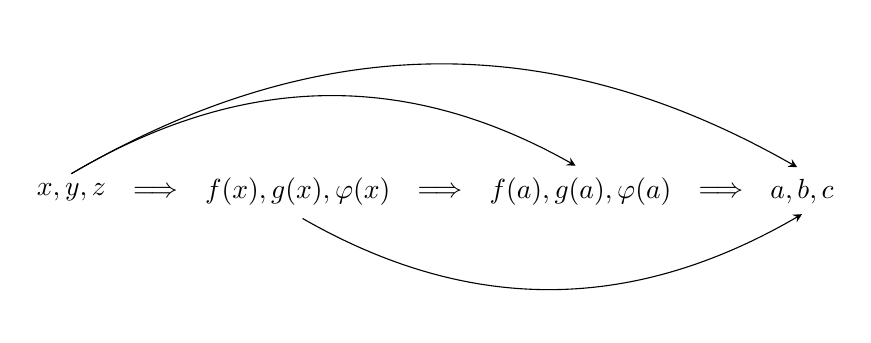
\begin{tikzpicture}
  \node (one) {$x,y,z$};
  \node[right=0cm of one] (one1) {$\implies$};
  \node[right=0cm of one1] (two) {$f(x),g(x),\varphi(x)$};
  \node[right=0cm of two] (two1) {$\implies$};
  \node[right=0cm of two1] (three) {$f(a),g(a),\varphi(a)$};
  \node[right=0cm of three] (three1) {$\implies$};
  \node[right=0cm of three1] (four) {$a,b,c$};
  \draw[-stealth,shorten >= 2pt] (one.north) to[bend left] (three.north);
  \draw[-stealth,shorten >= 2pt] (one.north) to[bend left] (four.north);
  \draw[stealth-,shorten >= 2pt] (four.south) to[bend left] (two.south);
  % \draw[-stealth,shorten >= 2pt] (three.south) to[bend left] node[below] {4} (two.south);
\end{tikzpicture}

\end{center}
\end{document}
